%%%%%%%%%%%%%%%%%%%%%%%%%%%%%%%%%%%%%%%%%%%%%%%%%%%%%%%%%%%%
%% ERBPI
%%%%%%%%%%%%%%%%%%%%%%%%%%%%%%%%%%%%%%%%%%%%%%%%%%%%%%%%%%%%


La idea general del software es que permita, a trav�s de una interfaz gr�fica y sencilla,
programar los robots para realizar distintas experiencias de veh�culos de Braitenberg y 
comportamiento basado en subsumisi�n\footnote{\textit{Subsumption Architecture}, Behavior-Based Robotics, R. C. Arkin.}.

Para eso, nos basamos en el survey que realizamos, principalmente los programas \textit{StarLogo} y \textit{Scratch}, 
que resultaron los mejorcitos en cuanto a la interfaz gr�fica de programaci�n y la idea de la interfaz gr�fica de proveer menus y submen�es con los objetos predefinidos para ir agregando...

La idea es poder combinar \textit{Braitenberg} y \textit{Subsumisi�n}, de manera que cada estado de la maquina de estados de subsimisi�n sea un braitenberg.
Entonces, en principio, se puede hacer s�lo Braitenberg. Luego, se puede hacer Subsumisi�n ``insertando'' en cada estado un braitenberg 
definido anteriormente.

Algo as� como la Figura \ref{Fig:subsumision}:

\begin{figure}
	\centering
	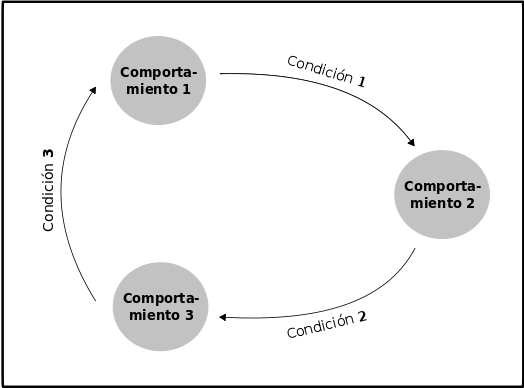
\includegraphics[scale=0.7]{images/subsumision.png}
	\caption{FORMA GENERAL DISE\~nO SOFTWARE.}
	\label{Fig:subsumision}
\end{figure}

ARREGLAR ESTO, COMPLETAR CON LO DEL EUROBOT2011 QUE EST\'A MUY BIEN...